\chapter{SegRanks Application Development Documentation}
\label{chapter:implementation}

\textit{SegRanks} is a Django web application which follows the standard
Django's structure and guidelines. It uses Model-View-Controller (MVC) pattern,
although in Django, views are called templates and controllers are called
views. We will use the Django's terminology here.

The model describes the representation of the data stored in the database.
Views prepare the data that gets presented to the user and also process user
requests and updates the data. Templates describe how the presented data will
look.

\section{Model}

The Django's object-relational mapping (ORM) is used to access the data in the
database. It allows to manipulate with data using an object interface. There
is no need to write SQL queries manually, all manipulations with data objects are
translated to SQL automatically on background. 

The database model is implemented in \texttt{segranks/model.py} using the
Django's model API. You can see the model illustrated in Figure \ref{model}.

Annotation projects are stored in table \textit{RankProject}. Each project
contains a number of sentences stored in table \textit{Sentence}, together with
reference translations. 

All extracted segments of a sentence are stored in table \textit{Segment}.
This table has two important fields. The first is \textit{candidates\_str},
which stores tab separated strings of all candidate translations of the
segment.  Although this is not a normalized design, it makes a lot of things
much simpler (all the candidates are ranked at once anyway).  The second field
is \textit{segment\_indexes} which stores the indices of words of the segment
in the source sentence.  This is used for highlighting the segment in the
interface.

Finally, each segment has zero or more annotations stored in
\textit{Annotation} table. When an annotation is submitted to the server, a new
row for each segment in the sentence is created in this table. The most
important field in this table is \textit{ranks} which stores ranks of the
segment candidates separated by tabs as a string. The reason for breaking the
database normalization is the same as before. There are convenient getters and
setters for these unnormalized data, so this is only an implementation detail,
hidden from the rest of the application. The table also stores some metadata
(who created the annotation, how long did it take, etc.).

Because there were some changes of the database model during the development,
we use \textit{South} to track the database changes and easily migrate the
data.

\begin{figure}
    \begin{center}
        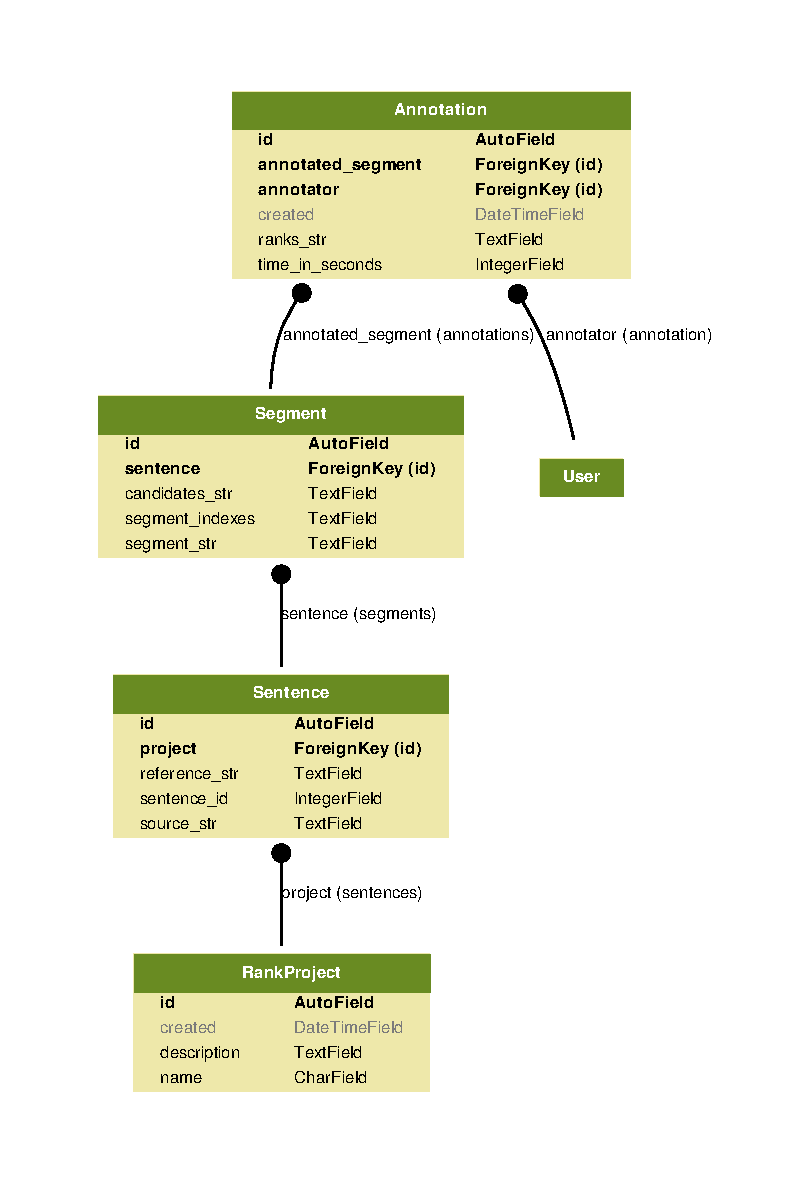
\includegraphics[width=12cm]{img/model.pdf}
    \end{center}

    \caption{Database model}
    \label{model}
\end{figure}

\section{Views}

Application URLs are mapped to individual views in file
\texttt{segranks/views.py}. All views are implemented as classes in file
\texttt{segranks/views.py}. There are three important views.

The simplest one is \textit{ProjectListView}, which lists all available
annotation projects. It is implemented as a subclass of Django's generic
\textit{ListView} class and does not implement any method.

\textit{AnnotateView} chooses a sentence to be annotated. This view is
implemented as a subclass of generic \textit{DetailView} class which renders a
single object. The only implemented method here is \textit{get\_object} which
returns a \textit{Sentence} object to be rendered. This method ensures that
annotators are sometimes shown already annotated sentences (for the computation
of agreements). In most of the cases, it simply choose a random unannotated
sentence.

The last view is \textit{SubmitView}. This view processes annotated sentences
submitted by annotators back to server. The ranks and other data are extracted
from the POST data and \textit{Annotation} instances are created for each
annotated segment. After that, the user is redirected to \textit{AnnotateView}
to get a new sentence to annotate.

There are also views which handle user registrations and logins, however these
views are part of the \textit{django-registration} library.

\section{Templates}

All templates are located in directory \texttt{segranks/templates}. The
\texttt{base.html} template contains all the elements which are common for all
templates (HTML head with links to client scripts and cascade styles, common
navigation bar) and other templates derive from it. Other templates contain
HTML code specific to views which they render.

The templates use \textit{Twitter Bootstrap} framework to easily build a simple
and responsive user interface. We also use \textit{jQuery} for easy element
selection and manipulation and for event handling. The drag-and-drop feature is
implemented using \textit{jQuery UI Sortable} widget.




